Um den Zeeman-Effekt zu erklären, wird hier zunächst auf die Drehimpulse der Elektronen in einem Atom eingegangen, die zu magnetischen Momenten führen und schlussendlich die Aufspaltung der Energieniveaus in einem Magnetfeld bewirken. Dann wird ausführlich darauf eingegangen, was beim Zeeman-Effekt beobachtet werden kann. Die theoretischen Grundlagen werden am Beispiel von Cadmium erklärt, das in diesem Versuch verwendet wird.

\subsection{Magnetisches Moment von einem Atom}
Der gesamte Drehimpuls $\vec{j}$ eines einzelnen Hüllenelektrons setzt sich aus dem Spin $\vec{s}$ und dem Bahndrehimpuls $\vec{l}$ zusammen. Wie aus der klassischen Mechanik bekannt führt ein elektrischer Kreisstrom zu einem magnetischen Moment. Dieses Phänomen ist allerdings nur als Analogon der klassischen Mechanik zur Quantenmechanik zu sehen. Das Elektron hat ein magnetisches Moment, das vom Spin generiert wird, $\vec{\mu}_s$ und eines, das vom Bahndrehimpuls herrührt $\vec{\mu}_l$. Beide magnetischen Momente zeigen entgegengesetzt zum entsprechenden Drehimpuls und sind proportional zum Betrag der Drehimpulse. Der Betrag vom Spin und vom Bahndrehimpuls kann durch die diskreten Quantenzahlen $s$ und $l$ ausgedrückt werden.
\begin{align}
	| \vec{s} | &= \sqrt{s(s+1)} \hbar \\
	| \vec{l} | &= \sqrt{l(l+1)} \hbar
\end{align}
Die magnetischen Momente sind 
\begin{align}
	\vec{\mu}_s &= - g_s \mu_B  \sqrt{s(s+1)} \vec{e}_s \\
	\vec{\mu}_l & = - \mu_B  \sqrt{l(l+1)} \vec{e}_l 
\end{align}
mit den Einheitsvektoren $\vec{e}_s$ und $\vec{e}_l$, dem Landé-Faktor $g_s$ (für ein freies Elektron gilt~$g_s \approx 2$) und dem Bohrschen Magneton \\
\begin{equation}
	\mu_B =- \frac{e_0 \hbar}{2 m_0}  \quad .
\end{equation}
Gibt es nun mehr als ein Hüllenelektron, so wechselwirken die Spins und Bahndrehimpulse und addieren sich zu einem Gesamtdrehimpuls $\vec{J}$ aller Hüllenelektronen. Es lasse sich zwei Grenzfälle betrachten: Bei Atomen mit niedriger Kernladungszahl gilt die $LS$-Kopplung
\begin{align}
	\vec{J} = \vec{L} + \vec{S} = \sum_i \vec{l}_i + \sum_i \vec{s}_i \quad .
\end{align}
Wenn die Kernladungszahl groß ist, dominiert die Wechselwirkung zwischen den einzelnen Spins und Bahndrehimpulsen. Es gibt keinen Gesamtspin oder Gesamtbahndrehimpuls mehr, sonder nur noch einen Gesamtdrehimpuls. Man spricht von der $j$-$j$-Kopplung mit
\begin{align}
	\vec{J} = \sum_i \vec{j}_i = \sum_i \left( \vec{l}_i + \vec{s}_i \right) \quad .
\end{align}
Bei Atomen mit mittlerer Kernladungszahl existiert ein kontinuierlicher Übergang zwischen den Extremfällen. In diesem Versuch wird Cadmium untersucht. Cadmium hat die Kernladungszahl $Z = 48$ und fällt unter die $LS$-Kopplung. Um das gesamte magnetische Moment zu berechnen ist nur die nicht abgeschlossene Elektronenhülle relevant, da abgeschlossene Schalen keinen Gesamtdrehimpuls haben. Das gesamte magnetische Moment setzt sich also aus dem magnetischen Moment des Gesamtspins und des Gesamtbahndrehimpulses zusammen
\begin{align}
	\vec{\mu} = \vec{\mu}_L + \vec{\mu}_S  \quad .
\end{align}
Das magnetische Moment $\vec{\mu}$ ist wegen des Lande-Faktors des Spins nicht mehr parallel zum Gesamtdrehimpuls $\vec{J}$. Es ist aber die Projektion von $\vec{\mu}$ auf $\vec{J}$ relevant. Geometrische Überlegungen ergeben dann 
\begin{align}
	\vec{\mu}_J = \mu_B g \sqrt{J(J+1)} \vec{e}_J
\end{align}
mit dem Landé-Faktor
\begin{align}
g =	\frac{3J(J+1) + S(S+1) - L(L+1)}{2J(J+1)} \quad .
\end{align}
Hierbei ist $J$ die Quantenzahl des Gesamtdrehimpulses, $L$ die des Gesamtbahndrehimpulses und $S$ die des Gesamtspins.

\subsection{Normaler Zeeman-Effekt}\label{sec:normaler}
Beim normalen Zeeman-Effekt ist der Gesamtspin $S$ null. Der Effekt beschreibt folgendes: Ein magnetisches Moment in einem Magnetfeld $\vec{B}$ hat eine Energie, wenn das magnetische Moment parallel zu den Magnetfeldlinien ausgerichtet ist oder zumindest parallele Anteile hat. Der parallele Anteil des magnetischen Momentes kann nur diskrete Werte annehmen. Man spricht von der Richtungsquantelung. Die Orientierungsquantenzahl $m_J$ zu $J$ in Richtung des Magnetfeldes nimmt die Werte $J$, $J-1$ bis $-J$ an. Die Energie ist dann
\begin{align}
	E = - \vec{\mu}_J \cdot \vec{B} = m_J g \mu_B B \quad .
\end{align}
 Es erfolgt eine Aufspaltung der Energieniveaus mit den Energiedifferenzen
\begin{align}\label{eq:Energieverschiebung}
	dE = g\mu_B B \quad .
\end{align}
Der Landé-Faktor ist für alle Übergänge beim normalen Zeeman-Effekt identisch, da der Spin verschwindet und $J = L$ ist,  gilt 
\begin{align}
	g = 1 \quad .
\end{align}
Übergänge von Elektronen zwischen den Niveaus sind möglich, wenn die Übergänge die Auswahlregel $\Delta m_J = 0, \pm 1$ erfüllen. Zur Herleitung der Auswahlregel betrachtet man eine Superposition von zwei Lösungen der zeitabhängigen Schrödinger-Gleichung. Dieses Gesamtlösung $\psi(\vec{r}, t) = c_\alpha \psi_\alpha + c_\beta \psi_\beta$ hat einen Ortsanteil und einen Zeitanteil. Die Dichtefunktion $\int \psi^{*}\psi \dd V$ ist zeitabhängig. Das Elektron schwingt und erzeugt so einen elektrischen Dipol mit den charakteristischen Matrixelementen der Übergänge:
\begin{align}
	x_{\alpha \beta} = \int x \psi_\alpha^{*}\psi_\beta \dd V \quad
	y_{\alpha \beta} = \int y \psi_\alpha^{*}\psi_\beta \dd V \quad
	z_{\alpha \beta} = \int z \psi_\alpha^{*}\psi_\beta \dd V
\end{align}
Die Matrixelemente stehen in Zusammenhang mit dem Pointing-Vektor, der die Richtung des Energietransportes der Welle angibt. Nur für die Übergänge  $\Delta m_J = 0, \pm 1$ findet ein Energietransport statt.
\\Das Elektron gewinnt durch den Übergang in ein niedrigeres Energieniveaus Energie und strahlt  eine elektromagnetische Welle mit der Frequenz $\nu= \Delta E / h $ ab. Für $\Delta m_J = 0$ strahlt das Elektron linear polarisiertes Licht ($\pi$-Übergang) ab und für $\Delta m = \pm 1$ zirkular polarisiertes Licht ($\sigma_{\pm}$-Übergang). 
Die Übergänge unterschiedlicher Polarisation können nur in bestimmten Beobachtungsrichtungen zum Magnetfeld gesehen werden. Das linear polarisierte Licht ist sichtbar, wenn man den Anteil beobachtet, der parallel zu den Magnetfeldlinien steht und den zirkular polarisierten Anteil entsprechend bei der Betrachtung des senkrechten Anteils, siehe Abb. \ref{fig:abb4}. Der Grund dafür ist die Ausrichtung des Dipols zum Magnetfeld.
\begin{figure}
	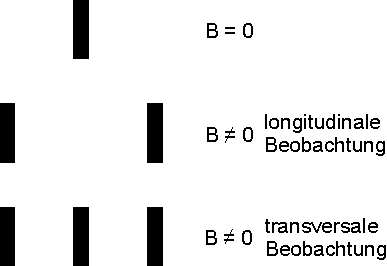
\includegraphics[width = 0.4\textwidth]{Abb4.pdf}
	\caption[Polarisationsrichtung]{Aufspaltung des Energieniveaus für $J=1$ in Abhängigkeit der Beobachtungsrichtung des ausgestrahlten Lichtes \cite{\V}}
	\label{fig:abb4}
	\end{figure}
\subsubsection{Cadmium -- rote Spektrallinie $\lambda = \SI{643.8}{\nano\meter}$}
Bei dem Übergang von dem Niveau $\ce{^1D_2}$ auf das Niveau $\ce{^1P_1}$ entsteht eine rote Spektrallinie mit einer Wellenlänge von $\lambda = \SI{643.8}{\nano\meter}$. Die Quantenzahlen der Niveaus sind:
\begin{align}
	&\ce{^1D_2} : \quad L=1, J =1, S =0 \notag \\
	&\ce{^1P_1}: \quad L = 2, J = 2, S = 0 \notag
\end{align}	
Der Landè-Faktor ist immer $g=1$. Es sind neun verschiedene Übergänge möglich (siehe Abbildung \ref{fig:mausi1} und Tabelle \ref{tab:g}). Es gilt
\begin{align}
	\Delta E &= \left( m_{J,1} g_1(L_1, S_1, J_1) - m_{J,2} g_2(L_2, S_2, J_2)  \right) \mu_B B \notag \\
	& =g_{12} \mu_B  B
\end{align}
mit
\begin{align}
	g_{12} = m_{J,1} g_1(L_1, S_1, J_1) - m_{J,2} g_2(L_2, S_2, J_2)  \quad .
\end{align}
\begin{figure}
	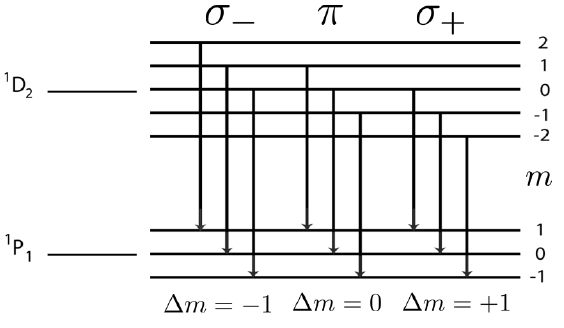
\includegraphics[width = 0.4\textwidth]{Mausi1.png}
	\caption[Aufspaltung von $\ce{^1D_2}$ auf $\ce{^1P_1}$]{Aufspaltung mögliche Übergänge  von Niveau $\ce{^1D_2}$ auf das Niveau $\ce{^1P_1}$. \cite{V27_mausi}}
	\label{fig:mausi1}
\end{figure}
\begin{table}
	\begin{tabular}{cccccc}
		& $m_1$ & $g_1$ & $m_2$ & $g_2$ & $g_{12}$ \\
		\hline
		$\sigma_-$ & -1 & 1& 0 & 0 & -1 \\
		& 0 & 1 & 1 & 1 & -1 \\
		& 1 & 1 & 2 & 1 & -1 \\
		\hline
		$\pi$ & -1 & 1 & -1 & 1 & 0 \\
		& 0 & 1 & 0 & 1 & 0 \\
		& 1 & 1 & 1 & 1 & 0 \\
		\hline
		$\sigma_+$  & -1 & 1 & 0 & 1 & 1 \\
		& 0 & 1 & -1 & 1 & 1 \\
		& 1 & 1 & -2 & 1 & 1
	\end{tabular}
	\caption[Normaler Zeeman-Effekt $g_{12}$]{Berechnung der Faktoren $g_{12}$ bei dem Übergang von Niveau $\ce{^1D_2}$ auf das Niveau $\ce{^1P_1}$.}
	\label{tab:g}
\end{table}

\subsection{Anormaler Zeeman-Effekt}
Der anormale Zeeman-Effekt unterscheidet sich vom normalen Zeeman-Effekt dadurch, dass der Gesamtspin $S$ von null verschieden ist. Der anormale Zeeman-Effekt tritt häufiger auf als der normale Zeeman-Effekt. Die Auswahlregel für die Übergänge $\Delta m_J = 0, \pm 1$ gilt weiterhin und auch die Polarisation der emittieren Welle ist genau wie beim normalen Zeeman-Effekt (siehe Kaptiel \ref{sec:normaler}). Die Energiedifferenzen zwischen den Niveaus sind hingegen nicht mehr äquidistant, da der Landé-Faktor der einzelnen Niveaus unterschiedlich ist.
\subsubsection{Cadmium -- blaue Spektrallinie $\lambda = \si{480}{\nano\meter}$}
Der Übergang von dem Niveau $\ce{^3P_1}$ auf das Niveau $\ce{^3S_1}$ erzeugt eine blaue Spektrallinie mit einer Wellenlänge von $\lambda = \si{480}{\nano\meter}$. Die Quantenzahlen der Niveaus sind
\begin{align}
	&\ce{^3P_1} : \quad L=1, J =1, S =1 \notag \\
	&\ce{^3S_1}: \quad L = 0, J = 1, S = 1 \notag
 \end{align}	
Die Übergänge sind in Abbildung \ref{fig:mausi2} dargestellt und die Faktoren $g_{12}$ sind in Tabelle~\ref{tab:g12} zu finden.

\begin{figure}
	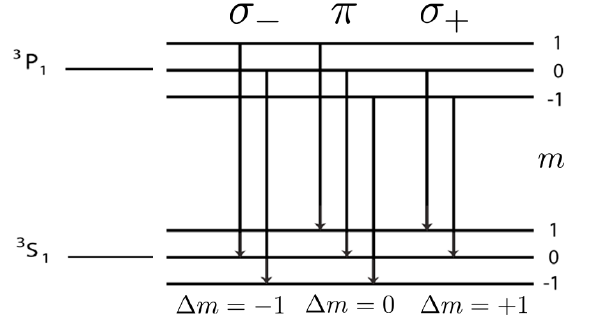
\includegraphics[width = 0.4\textwidth]{Mausi2.png}
	\caption{Mögliche Übergänge  von Niveau $\ce{^3P_1}$ auf das Niveau $\ce{^3S_1}$. \cite{V27_mausi}}
	\label{fig:mausi2}
\end{figure}

\begin{table}
\begin{tabular}{cccccc}
	& $m_1$ & $g_1$ & $m_2$ & $g_2$ & $g_{12}$ \\
	\hline
	$\sigma_-$ & -1 & 2& 0 & 1.5 & -2 \\
	& 0 & 2 & 1 & 1.5 & -1.5 \\
	\hline
	$\pi$ & -1 & 2 & -1 & 1.5 & -0.5 \\
	& 0 & 2 & 0 & 1.5 & 0 \\
	& 1 & 2 & 1 & 1.5 & 0.5 \\
	\hline
	$\sigma_+$ & 0 & 2 & -1 & 1.5 & 1.5 \\
	& 1 & 2 & 0 & 1.5 & 2
\end{tabular}
\caption[Anormaler Zeeman-Effekt $g_{12}$]{Berechnung der Faktoren $g_{12}$ bei dem Übergang von Niveau  $\ce{^3P_1}$ auf das Niveau $\ce{^3S_1}$.}
\label{tab:g12}
\end{table}




